\subsection{Neural network architecture and training}
\label{sec:architechture-and-training}

In this Section we describe the architecture of the CNN we adopt and how data are handled.
%
The input of the CNN are synthetic foreground-subtracted flux maps, and the output vector ${\hat y}_i = (\dnds|_j, \fiso)$ contains the reconstructed $\dnds|_j$ in 20 flux bins in {$[5 \cdot 10^{-12}, 1 \cdot 10^{-7}]$} cm$^{-2}$ s$^{-1}$, plus the reconstructed value of $\fiso$. The index $i$, thus, has values $i=1,...,21$.
A possible alternative would be to choose as output
the breaks and the slopes of the $\dnds$, i.e., the same parameters used to model the input $\dnds$. Nonetheless, we found a better stability of the CNN using as output directly the $\dnds$ function as discretized above, and we will thus use this as output. 

As further described below, we will use an approach in which we will let the CNN determine also the errors on the output parameters. The output vector will thus be effectively doubled. Beside the ${\hat y}_i$, we thus have also $\hat{\sigma}_i$ the output vector of the errors. 


Since we are dealing with sky maps, we can approach the problem from the point of view of image analysis. However, the image here is in spherical projection. We therefore need to adopt a method able to deal with this situation.


\subsubsection{Spherical neural networks}
In the last years, the machine learning community has realised the importance of developing neural network architectures on complex topologies. One of the most interesting non-trivial domains is that of a sphere, since it cannot be mapped on a plane without introducing distortion. This is the case we are confronting here, since we are dealing with sky maps.  There are many efforts to implement CNN architectures that can do convolutions on the sphere \cite{DBLP:journals/corr/abs-1708-00919,DBLP:journals/corr/abs-1902-04615,DBLP:journals/corr/abs-2012-15000,nnhealpix,mapped-convolutions}, and while there have been many proposals, there is not yet agreement on a standard algorithm.

In dealing with information extraction from spherical images, one has to cope with a set of issues: 
i) the algorithm needs to properly deal with the topology of the sphere without distorting the image or losing information;
ii) the algorithm has to be computationally efficient;
iii) it would be desirable to be able to use the same neural network architectures which already work for flat images, which have been proven to be very efficient and effective.

In fact, a full spherical architecture is usually slower than a flat architecture when applied to images of the same size, and it often happens that it is not possible to adopt pre-existing models without re-implementing them \textit{ad-hoc}. 
On the other hand, the adoption of a flat-image architecture either introduces spherical distortions, due to the mapping of a spherical image on a plane, or may loose some of the large scale information contained in the image.

In this work, we  implemented a fast and reliable spherical architecture on the Healpix pixelisation of the sphere, taking inspiration from the idea proposed in \cite{mapped-convolutions} for the icosahedron. This method proved to be reliable when the information we need to retrieve from the maps is a small-scale effect, like in our case the distribution of sources, which are point-like (although smeared by the PSF) and isotropically distributed.


The method is based on the fact that, in the Healpix pixelisation scheme, each pixel has equal area and contains the information of the underlying field (in our case, the photon counts) averaged over that pixel. As discussed above, we train our neural network on maps of order $n=6$ ($N_\textrm{side}=64$), which contain 49152 pixels. Considering instead the Healpix sphere with base pixelisation  of order $n=0$ ($N_\textrm{side}=1$), we can subdivide the map into 12 equal-area patches, each of which containing 4096 pixels. Each patch is an independent realisation of the underlying isotropic field and can be mapped into a 2D flat image. We call this parsing algorithm \verb|map2patch|. Notice that this is not a re-sampling of the map: it's just a subdivision of the spherical image into 12 patches, in a way that preserves the area and content of each pixel. This allows us to use standard convolutional network techniques that work efficiently on flat images, while preserving the whole available statistics of the full map.  


Convolution is performed on each patch separately. In order to be able to extract information from each patch in parallel, we define 3D convolutions, where the first two dimensions are the spatial dimensions, and the third dimension specifies the patch. In order to force the neural network to learn from each individual sky patch, we employ convolution filters of size $(N,N,1)$, where $N$ is the dimension of the filter. By doing so, we effectively apply 2D filters to the whole sky. Note that by employing such filter size, the output of each convolution will still have 12 separate images on the third axis, associated to each sky patch, while the number of channels will vary according to the number of filters employed. This technique will thus naturally scale for images with different color channels, such as RGB images, or spherical images for which several channels are available, as is the case where multiple energy bands are considered at once.

{  We stress that with our method we partially loose large-scale information and information stored at the border of the patches.
Thus our algorithm would not be suitable in the case one is interested in recovering large-scale features.
In our case, however, we are interested in exploring information which is  statistically isotropic and/or lies at scales much smaller then the size of a patch. In this case our architecture is certainly viable and extremely efficient.}
%but we do not alter the small-scale information contained in the pixels of individual patches. On the other hand, if the resolution is high enough and the information we are interested in exploring is isotropic and/or lies at scales much smaller then the size of a patch, this architecture is viable and extremely efficient. 
Also, since  we  build our patch on the pixels of the Healpix pixelisation scheme, there is no spherical distortion in our images, unlike other architectures which employ the euclidean projection of the sphere.

This approach is extremely fast, since it leverages on optimised 3D convolutions. Furthermore the sphere-to-patch operation is performed asynchronously by the CPU while the accelerator is training the model, allowing for virtually no bottlenecks in the processing pipeline.

In order to cross-check our method, we also implemented the full-sky truly-spherical convolutions of \cite{nnhealpix}, obtaining very similar results. {  In  Appendix \ref{sec:full-spherical-nn}, we report some examples of the results and checks performed with a fully spherical convolution model.} The two methods are therefore interchangeable for the type of information we want extract from the \fermi maps: however, our implementation allowed us to gain more than a factor of 10 in time of execution of the whole pipeline of training and validation. This convergence of results with the fully spherical method of \cite{nnhealpix} gives us confidence on the reliability of our model, and the speed gain sets the basis for a future efficient extension of our analysis to several energy bins in the full \fermi energy range, in order to determine also the energy dependence of the $\dnds$  of unresolved sources.


\subsubsection{Data pre-processing}
\label{sec:preprocessing}

The maps are constructed with the procedure outlined in Section \ref{sec:generation}. As explained more in detail there, even though we apply a latitude cut to the maps, in order to further reduce the impact of the galactic foreground (and as it is customary in analyses of the extragalactic gamma-ray background), we subtract the galactic foreground (normalized by the $A_\textrm{gal}$ constant) from the input maps. This will also facilitate to some extent the training of the CNN, whose goal is to reconstruct the source-count distribution. Photon-counts maps are converted in units of flux, by using the exposure map. In order to reduce the variability of the inputs seen by the CNN and stabilize its behaviour, we take the logarithm of the flux values in the pixels and then map them in $[-1,1]$ range. 
Finally, each map is parsed into 12 patches using the \verb|map2patch| algorithm discussed in the previous Sections.

Given the approximate $S^{-2}$ behavior of the $\dnds$, for the output vector, we reconstruct $y_i = S^2 \dnds|_i \times 10^{11}$ cm$^{2}$ s deg$^{2}$ ($i=1,20$) and $y_{21}=\fiso \cdot  10^{7}$ cm$^{2}$ s sr, in order to work with (pure) numbers of order unity. We adopt this strategy in order to avoid that the mean square error could favour the optimisation of any flux bin over another, making the deviations more even across the range of $S$.

\subsubsection{Network architecture}
In recent years, we have seen the rise of many convolutional neural network models for computer vision tasks \cite{CNNreview1, CNNreview2, CNNreview3}.
Modern convolutional neural network architectures can have a very large numbers of internal parameters. This is due to the complex links between each neural unit, which allows for these models to be highly expressive and effectively behave as universal approximators for many kinds of tasks \cite{HORNIK1989359}. Unfortunately this comes with a downside: these models are prone to fitting too well the training dataset, which would lead to poorer performance on new data. In the field of Machine Learning, this problem is known as "overfitting" \cite{overfitting}. In order to prevent overfitting, 
a possible solution is to train the model on a big enough dataset.
This will render impossible for the NN to learn exactly the representation of the training set, as well as showing a richer feature space, which will result in better performance on any additional sample for which we may want to get a prediction, like the real case scenario with the Fermi photon counts map. Another solution is to apply regularisation layers which force the NN to learn a more general representation of the data, by promoting several metrics. Some of the most common regularisation techniques include L1 and L2 regularisation, batch normalisation, and dropout \cite{dropout, batch-normalization, regularisation1, regularisation2}.

We choose as our convolutional neural network architecture the EfficientNet V2M model \cite{efficient-net-v2}. This model has been proven to be faster to train then other models for computer vision tasks, while retaining the same expressivity and predictive power. 
Furthermore, its low memory footprint helps in training with more data at the same time (larger batch sizes), which in turn reduces the risk of overfitting.
In this work, following the original implementation of EfficientNet, we will adopt batch normalisation layers after each convolution.

We additionally employ a fairly new trainable implementation of dropout, called concrete dropout \cite{concrete-dropout}, before each convolution layer.
Dropout \cite{dropout} has been proven to be an efficient way to reduce overfitting in a model, by randomly turning off neurons or connections inside a model. Unfortunately, the dropout probability for each dropout layer has to be either hand picked or optimised through grid search, which is practically unfeasible for very large models. If the dropout probability is too small, the regularisation effect will not be very significant, while on the other hand too high a dropout probability will result in slower training and worse overall performance (underfitting). 
We therefore adopt the implementation of dropout as a concrete Bernoulli distribution \cite{concrete-distribution}, which allows the self-learning of the optimal dropout probability, effectively saving a conspicuous amount of time while training and ensuring that the model will be less prone to overfitting. 




\subsubsection{Bayesian error estimation and cost function}
\label{sec:bayesian-error}


In order to correctly estimate the error on a prediction, it is necessary to correctly estimate both the systematic error (sometimes called epistemic error \cite{epistemic-err}) and aleatory error components of a measurement. One way to estimate such components together is through a Bayesian approach, and in particular by defining a Bayesian neural network capable of estimating the posterior distribution of the desired observables.   
It has been shown \cite{mcdropout} 
that a NN with arbitrary depth and  non-linearities, with dropout applied before every weight layer, is mathematically equivalent to an approximation of a Bayesian model. 

In a subsequent analysis \cite{heteroscedastic-error} it has been shown how to estimate the first and second momenta (mean and variance) of the posterior distribution, under the assumption of a Gaussian likelihood of unknown variance. In particular \cite{heteroscedastic-error} shows how to define a neural network capable of determining the appropriate variances of such a multivariate Gaussian.
In our case, training a neural network with such an approach is advantageous, as the neural network will learn to weight less the component of the measurement at low fluxes, which we expect to be more uncertain, which helps in obtaining stable measurements for the test dataset. 

Following \cite{heteroscedastic-error} we define the heteroscedastic Gaussian negative log-likelihood:
\begin{equation}
    \textsl{NLL} = \sum_{i=1}^N  \left[\frac{(y_i^\textrm{true}-y_i^\textrm{pred})^2}{2\sigma_i^2} + \frac{1}{2} \log(\sigma_i^2)  +  \frac{1}{2} \log(2\pi)  \right]
\label{costfunc}    
\end{equation}
where we compare the true $\dnds$ and $\fiso$ (transformed as discussed in Section \ref{sec:preprocessing}) used to generate the simulated map with the prediction of the neural network, and thus $N=20+1$.
For the training of the neural network, we omit the last term of Eq. (\ref{costfunc}) which is an irrelevant constant.
%
Regarding the errors, since the first term in Eq. (\ref{costfunc}) is a decreasing function of the $\sigma_i$ while the second is increasing, this ensures that there will be a minimum which will provide the  optimal estimate for the $\sigma_i$ themselves.

In principle, the above cost function can easily be generalized to account for the covariance among the different bins and $F_\textrm{iso}$. 
 In practice, however, this implies estimating also the off-diagonal terms of a $21 \times 21$ symmetric matrix. Such matrix has to be inferred autonomously from data without any supervision, making the problem very challenging to optimise in this form. We thus refrain from attempting estimating the covariance. For CNN applications where the covariance between a set of parameters has been estimated, see e.g. Ref. \cite{Mishra-Sharma:2021oxe, List:2020mzd}.








\subsubsection{Training and validation}
\label{sec:NN-training}

\begin{figure}[t]
\centering
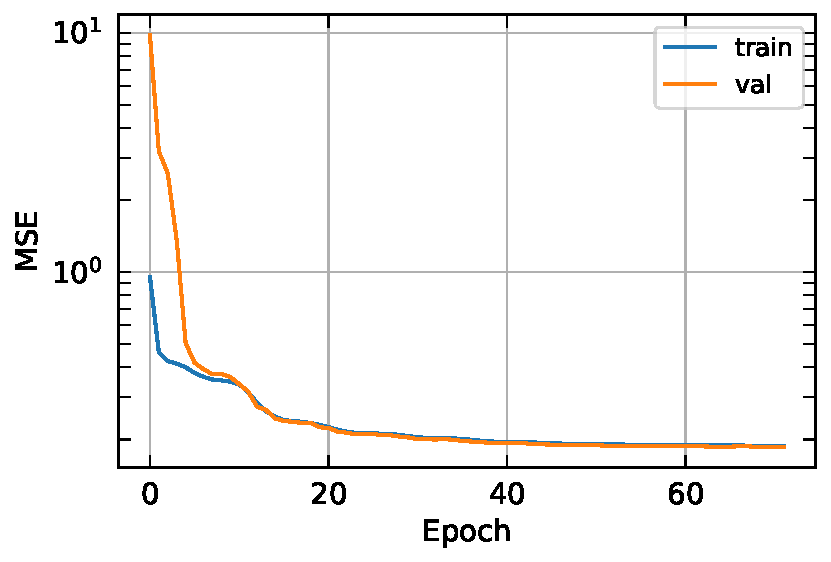
\includegraphics[width=0.6\textwidth]{chapter_06/sections/paper_dnds/img/model_plots/MSE.pdf}
\caption{ Epoch evolution of the MSE for the training (blue line) and validation (orange line) sets.}
\label{fig:mse-training}
\end{figure}

\begin{figure}[t]
\centering
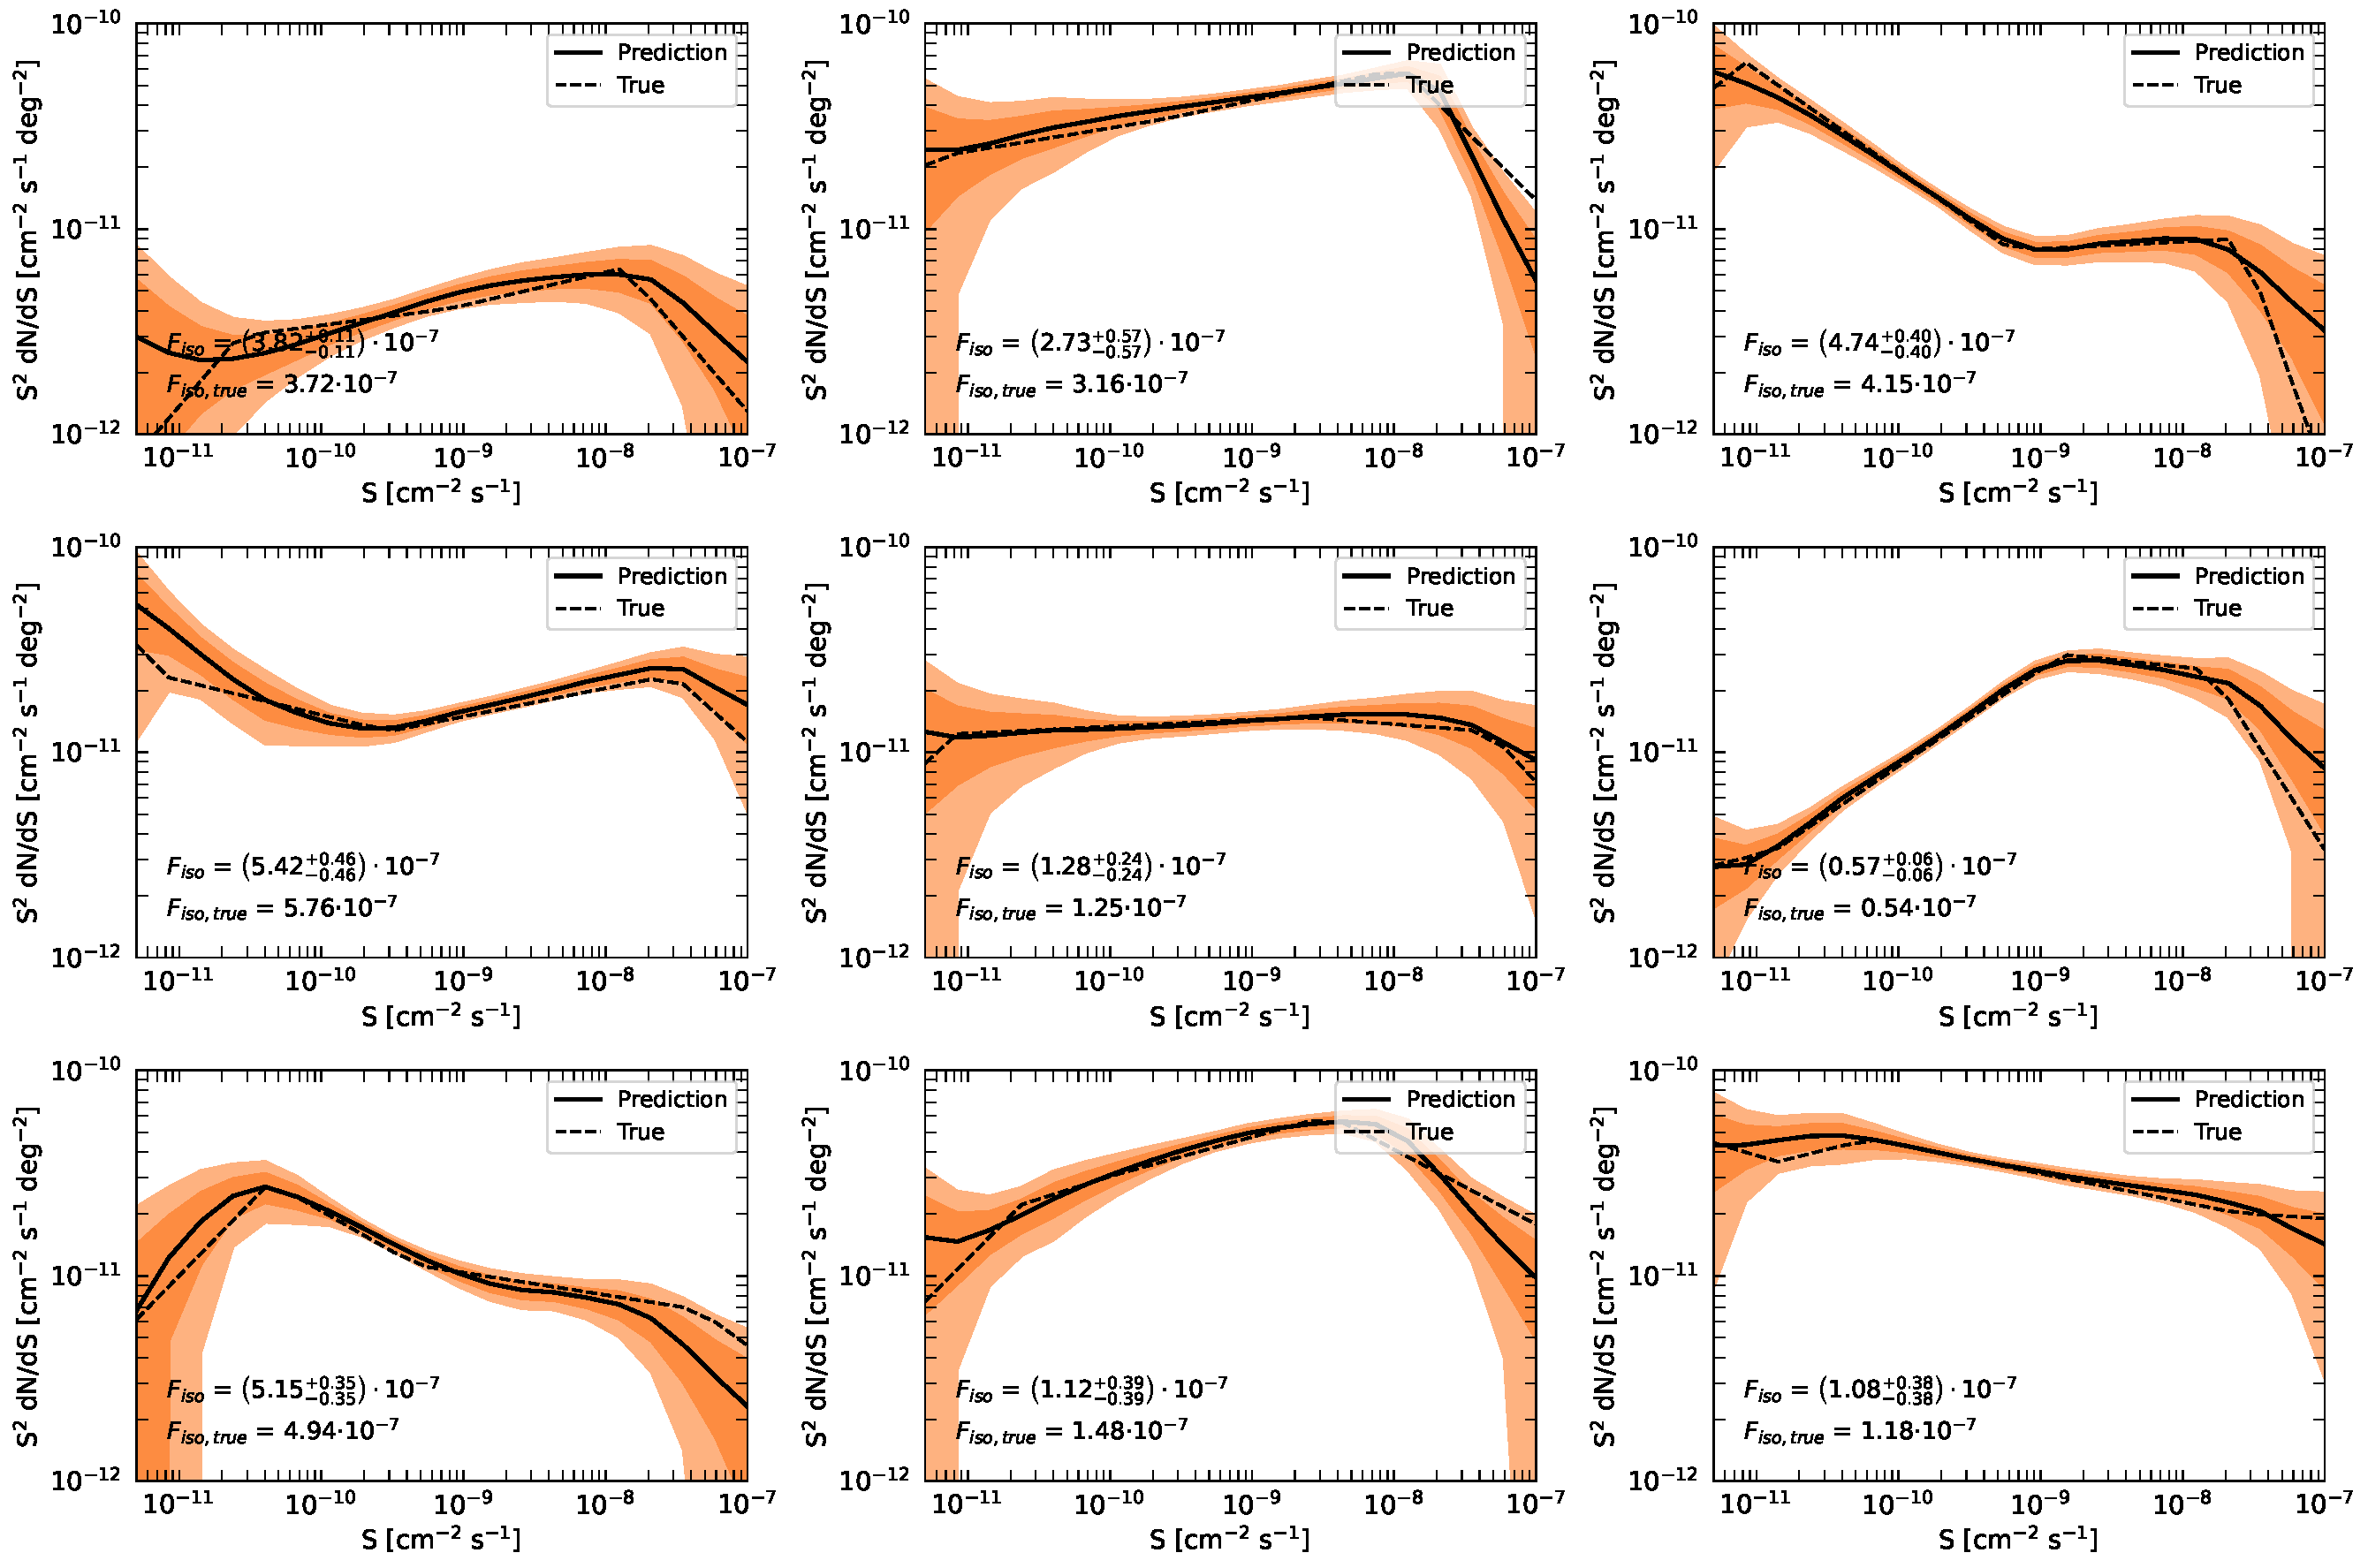
\includegraphics[width=1.0\textwidth]{chapter_06/sections/paper_dnds/img/model_plots/model_42/baseline/sample_maps.pdf}
\caption{Some example $\dnds$ from the validation dataset. Each panel shows the input $\dnds$ and $\fiso$ and the corresponding quantities reconstructed by the CNN. The colored bands indicate 1-2 $\sigma$ uncertainty regions. See text for more details. }
\label{fig:random-maps}
\end{figure}

We train our model using a Tensor Processing Unit (TPU) v3, kindly provided by the Google$^\textrm{TM}$ TPU Research Cloud. We adopt the Adam optimizer. We employ a cyclical triangular learning rate \cite{triangular} to avoid falling into local minima of the parameter space. We adopt a batch size equal to $128\times 8=1024$ to fully exploit the computational capabilities of the TPU. We train the model for 72 epochs, for a total of 9 triangular learning rate cycles, with learning rate ranging from $10^{-6}$ to $10^{-3}$. 
As already anticipated, we have generated 1 million maps, 90\% of which have been employed in the training and 10\% for validation.

To test the convergence of the model we evaluate the mean square error (MSE)  defined as $MSE=\sum_{i=1}^N (y_i^\textrm{true}-y_i^\textrm{pred})^2$. 
In Fig. \ref{fig:mse-training} we plot the MSE as a function of the training epoch for the training and validation dataset. We can see that, starting from epoch 10, the validation and training lines are close to each other, which means that our model is not overfitting the training dataset. We observe that the MSE reaches a plateau at around epoch 60, meaning that further training of our model would not lead to  improvement in performance.

Once the CNN is fully trained, we extensively check the convergence of the reconstructed $\dnds$ and $\fiso$ against their inputs, by using the maps of the validation set. 
Fig. \ref{fig:random-maps} shows a few illustrative examples of $\dnds$, randomly generated according to the priors and parameters intervals listed in Table \ref{tab:prior-dNdS}, together with their reconstructions. 
The dashed black lines show the input $\dnds$ and the black solid lines denote the corresponding distributions reconstructed by the CNN. The  input and reconstructed values of $\fiso$ are also quoted. The colored bands refer to the $1\sigma$ and $2\sigma$ confidence intervals
as estimated by the CNN.
The CNN recovers a $\dnds$ which is compatible with the input. The error bands are large for high fluxes, due to the fact that the number of sources at those values of $S$ is low and therefore a large statistical uncertainty is expected. The error band becomes large again at low fluxes, indicating that the CNN reaches a confusion limit: even though here the number of sources is very large, their faintness makes progressively harder to identify their number and a confusion between faint sources and the average isotropic component $\fiso$ arises, the lower the valus of $S$ becomes. This same behaviour also occurs in the 1point-PDF analysis of \cite{Cuoco-1pdf}. Concerning the value of $\fiso$, the reconstruction is very good, compatible with the input and with a small uncertainty. 



\subsubsection{Frequentist error estimation and Bias}
\label{sec:bias}

\begin{figure}[t]
\centering
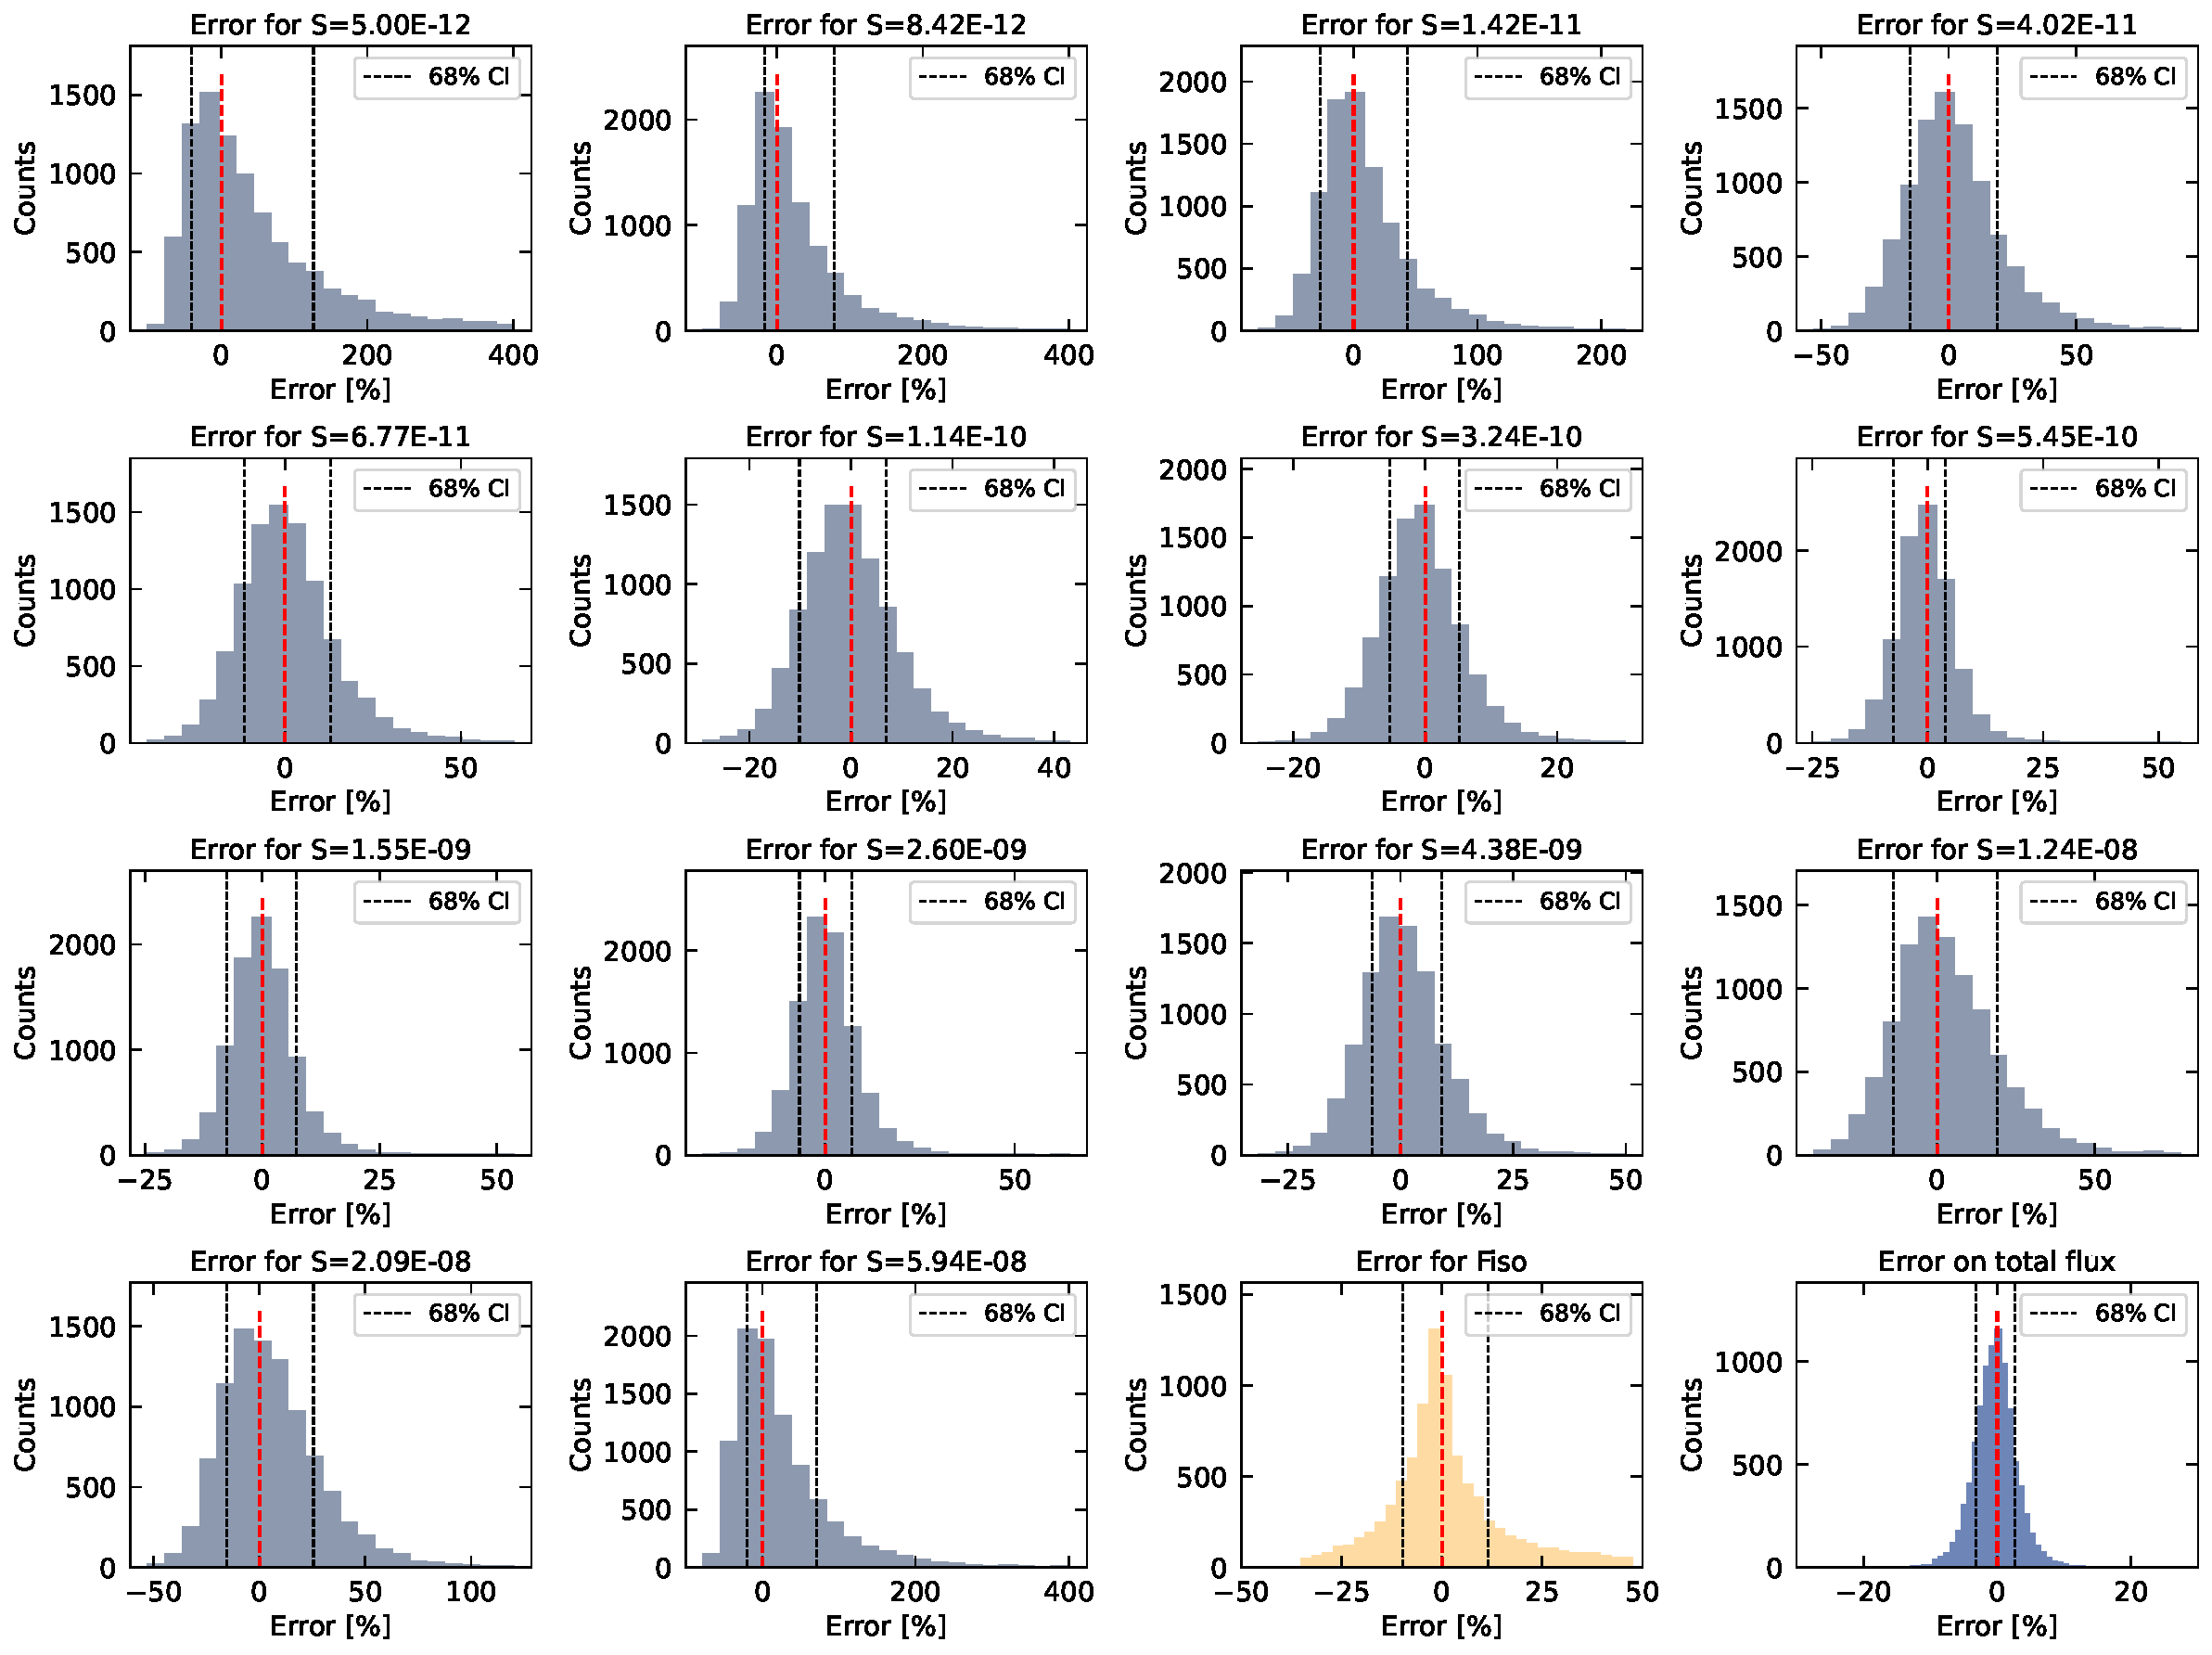
\includegraphics[width=1.0\textwidth]{chapter_06/sections/paper_dnds/img/model_plots/model_42/baseline/model_42_7e2_n64_flat_HL_error_histogram.pdf}
\caption{ Histograms of the percentage deviations between the true and reconstructed $\dnds$ for 14 values of $S$ across its interval of interest, and for $\fiso$. The bottom right panel shows the same, but for a derived quantity, namely the total flux. The dotted vertical black lines indicate the 68\% confidence region.}
\label{fig:bias-histogram}
\end{figure}

\begin{figure}[t]
\centering
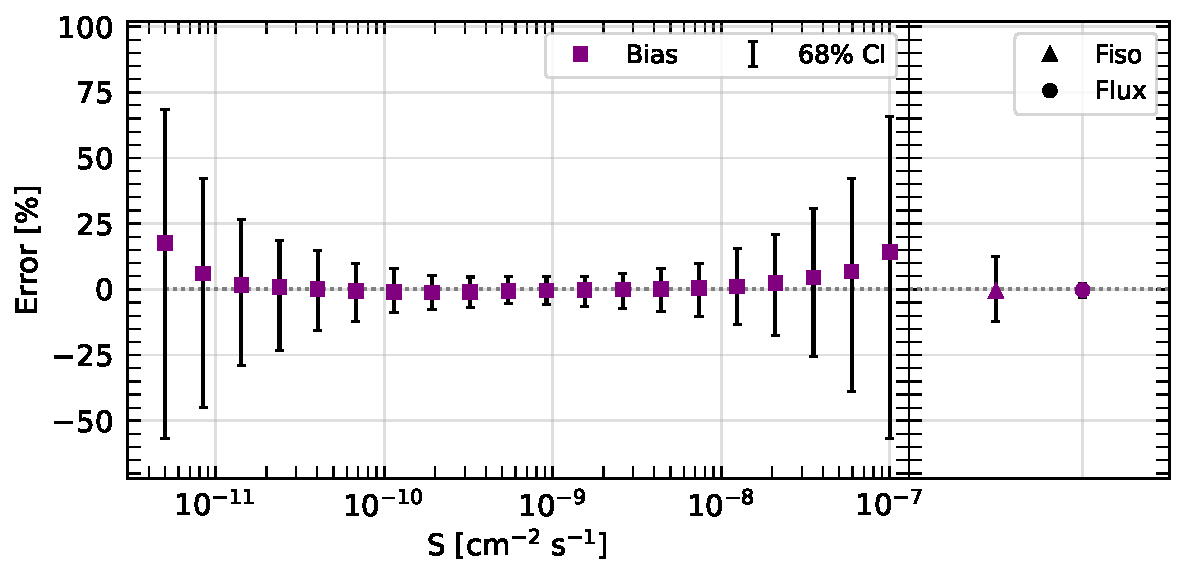
\includegraphics[width=0.8\textwidth]{chapter_06/sections/paper_dnds/img/model_plots/model_42/baseline/model_42_7e2_n64_flat_HL_dNdS_errors}
\caption{68\% error for the reconstructed $\dnds$ as function of $S$, for $\fiso$ and for the total flux. Also shown is the bias given by the median of the histogram for each $S$ bin (squares).
}
\label{fig:bias-plot}
\end{figure}

Besides the Bayesian error automatically provided as output by the CNN, we also estimate the error in an alternative frequentist-like way, in order to provide a cross-check. This second method gives as a further advantage also the possibility to estimate the amount of bias on the reconstructed $\dnds$.
To this aim, we have built, for each of the 20 bins in flux and for $\fiso$, the histogram of the deviations between the true and reconstructed $\dnds$  and $\fiso$. The results for 14 values of $S$ across its interval of interest, and for $\fiso$, are shown in Fig. \ref{fig:bias-histogram} (the remaining histograms are similar in content and are not shown here for economy of space). The plot shows the distribution of models which exhibit a specific relative deviation (expressed as percentage of the true value). By using these
distributions of the deviations (normalized to unity), we derived the $1\sigma$ and $2\sigma$ confidence level intervals on the reconstructed $\dnds$ and $\fiso$. As anticipated in Section \ref{sec:NN-training}, at low and large fluxes the distributions are wide, implying a poorer ability to reconstruct the underlying physical models, while in the flux interval $(1 \cdot 10^{-11}, 2 \cdot 10^{-8})$ cm$^{-2}$ s$^{-1}$ the $1\sigma$ error is below 30\%, with an error below 20\% for $S$ in $(1 \cdot 10^{-10}, 1 \cdot 10^{-8})$ cm$^{-2}$ s$^{-1}$. The $1\sigma$ error on $\fiso$ is also of the order of 20\%. The last panel of Fig. \ref{fig:bias-histogram} shows the histogram for the reconstructed value of the total photon flux: this is a sanity check and shows that the CNN correctly reproduces the normalization of the maps in terms of total counting rate. The uncertainty on the total flux is 5\%. The $1\sigma$ (non symmetric) intervals for all the 20 flux bins are also reported in Fig. \ref{fig:bias-plot}.
A more direct comparison of the Bayesian and frequentist errors is provided in the results section.

The same histograms of Fig. \ref{fig:bias-histogram} allow us also to check whether the reconstructed values are biased. We define the bias as the deviation between the median of the distribution and the input value. The values of the bias are shown, for each of the 20 values of flux, in Fig. \ref{fig:bias-plot} as squares. We see that for all fluxes, the bias is very close to zero, which implies that the reconstructed values not only are determined with good precision (since the error bar is small), but also without a  bias toward larger or lower values. The only exception is a positive bias for very low fluxes, where the CNN meets its confusion limit, and for very large fluxes, where the low source-counts statistics produces a small overestimate of the underlying $\dnds$.
In both cases, however, the bias is small compared to the overall error.

